\chapter{The Island of Monte Cristo}

Thus, at length, by one of the unexpected strokes of fortune which
sometimes befall those who have for a long time been the victims of an
evil destiny, Dantès was about to secure the opportunity he wished for,
by simple and natural means, and land on the island without incurring
any suspicion. One night more and he would be on his way.

The night was one of feverish distraction, and in its progress visions,
good and evil, passed through Dantès’ mind. If he closed his eyes, he
saw Cardinal Spada’s letter written on the wall in characters of
flame—if he slept for a moment the wildest dreams haunted his brain. He
ascended into grottos paved with emeralds, with panels of rubies, and
the roof glowing with diamond stalactites. Pearls fell drop by drop, as
subterranean waters filter in their caves. Edmond, amazed,
wonderstruck, filled his pockets with the radiant gems and then
returned to daylight, when he discovered that his prizes had all
changed into common pebbles. He then endeavored to re-enter the
marvellous grottos, but they had suddenly receded, and now the path
became a labyrinth, and then the entrance vanished, and in vain did he
tax his memory for the magic and mysterious word which opened the
splendid caverns of Ali Baba to the Arabian fisherman. All was useless,
the treasure disappeared, and had again reverted to the genii from whom
for a moment he had hoped to carry it off.

The day came at length, and was almost as feverish as the night had
been, but it brought reason to the aid of imagination, and Dantès was
then enabled to arrange a plan which had hitherto been vague and
unsettled in his brain. Night came, and with it the preparation for
departure, and these preparations served to conceal Dantès’ agitation.
He had by degrees assumed such authority over his companions that he
was almost like a commander on board; and as his orders were always
clear, distinct, and easy of execution, his comrades obeyed him with
celerity and pleasure.

The old patron did not interfere, for he too had recognized the
superiority of Dantès over the crew and himself. He saw in the young
man his natural successor, and regretted that he had not a daughter,
that he might have bound Edmond to him by a more secure alliance. At
seven o’clock in the evening all was ready, and at ten minutes past
seven they doubled the lighthouse just as the beacon was kindled. The
sea was calm, and, with a fresh breeze from the south-east, they sailed
beneath a bright blue sky, in which God also lighted up in turn his
beacon lights, each of which is a world. Dantès told them that all
hands might turn in, and he would take the helm. When the Maltese (for
so they called Dantès) had said this, it was sufficient, and all went
to their bunks contentedly.

This frequently happened. Dantès, cast from solitude into the world,
frequently experienced an imperious desire for solitude; and what
solitude is more complete, or more poetical, than that of a ship
floating in isolation on the sea during the obscurity of the night, in
the silence of immensity, and under the eye of Heaven?

Now this solitude was peopled with his thoughts, the night lighted up
by his illusions, and the silence animated by his anticipations. When
the patron awoke, the vessel was hurrying on with every sail set, and
every sail full with the breeze. They were making nearly ten knots an
hour. The Island of Monte Cristo loomed large in the horizon. Edmond
resigned the lugger to the master’s care, and went and lay down in his
hammock; but, in spite of a sleepless night, he could not close his
eyes for a moment.

Two hours afterwards he came on deck, as the boat was about to double
the Island of Elba. They were just abreast of Mareciana, and beyond the
flat but verdant Island of La Pianosa. The peak of Monte Cristo
reddened by the burning sun, was seen against the azure sky. Dantès
ordered the helmsman to put down his helm, in order to leave La Pianosa
to starboard, as he knew that he should shorten his course by two or
three knots. About five o’clock in the evening the island was distinct,
and everything on it was plainly perceptible, owing to that clearness
of the atmosphere peculiar to the light which the rays of the sun cast
at its setting.

Edmond gazed very earnestly at the mass of rocks which gave out all the
variety of twilight colors, from the brightest pink to the deepest
blue; and from time to time his cheeks flushed, his brow darkened, and
a mist passed over his eyes. Never did a gamester, whose whole fortune
is staked on one cast of the die, experience the anguish which Edmond
felt in his paroxysms of hope.

Night came, and at ten o’clock they anchored. \textit{La Jeune Amélie} was
first at the rendezvous. In spite of his usual command over himself,
Dantès could not restrain his impetuosity. He was the first to jump on
shore; and had he dared, he would, like Lucius Brutus, have “kissed his
mother earth.” It was dark, but at eleven o’clock the moon rose in the
midst of the ocean, whose every wave she silvered, and then, “ascending
high,” played in floods of pale light on the rocky hills of this second
Pelion.

The island was familiar to the crew of \textit{La Jeune Amélie},—it was one of
her regular haunts. As to Dantès, he had passed it on his voyage to and
from the Levant, but never touched at it. He questioned Jacopo.

“Where shall we pass the night?” he inquired.

“Why, on board the tartan,” replied the sailor.

“Should we not do better in the grottos?”

“What grottos?”

“Why, the grottos—caves of the island.”

“I do not know of any grottos,” replied Jacopo.

The cold sweat sprang forth on Dantès’ brow.

“What, are there no grottos at Monte Cristo?” he asked.

“None.”

For a moment Dantès was speechless; then he remembered that these caves
might have been filled up by some accident, or even stopped up, for the
sake of greater security, by Cardinal Spada. The point was, then, to
discover the hidden entrance. It was useless to search at night, and
Dantès therefore delayed all investigation until the morning. Besides,
a signal made half a league out at sea, and to which \textit{La Jeune Amélie}
replied by a similar signal, indicated that the moment for business had
come.

The boat that now arrived, assured by the answering signal that all was
well, soon came in sight, white and silent as a phantom, and cast
anchor within a cable’s length of shore.

Then the landing began. Dantès reflected, as he worked, on the shout of
joy which, with a single word, he could evoke from all these men, if he
gave utterance to the one unchanging thought that pervaded his heart;
but, far from disclosing this precious secret, he almost feared that he
had already said too much, and by his restlessness and continual
questions, his minute observations and evident preoccupation, aroused
suspicions. Fortunately, as regarded this circumstance at least, his
painful past gave to his countenance an indelible sadness, and the
glimmerings of gayety seen beneath this cloud were indeed but
transitory.

No one had the slightest suspicion; and when next day, taking a
fowling-piece, powder, and shot, Dantès declared his intention to go
and kill some of the wild goats that were seen springing from rock to
rock, his wish was construed into a love of sport, or a desire for
solitude. However, Jacopo insisted on following him, and Dantès did not
oppose this, fearing if he did so that he might incur distrust.
Scarcely, however, had they gone a quarter of a league when, having
killed a kid, he begged Jacopo to take it to his comrades, and request
them to cook it, and when ready to let him know by firing a gun. This
and some dried fruits and a flask of Monte Pulciano, was the bill of
fare.

Dantès went on, looking from time to time behind and around about him.
Having reached the summit of a rock, he saw, a thousand feet beneath
him, his companions, whom Jacopo had rejoined, and who were all busy
preparing the repast which Edmond’s skill as a marksman had augmented
with a capital dish.

Edmond looked at them for a moment with the sad and gentle smile of a
man superior to his fellows.

“In two hours’ time,” said he, “these persons will depart richer by
fifty piastres each, to go and risk their lives again by endeavoring to
gain fifty more; then they will return with a fortune of six hundred
francs, and waste this treasure in some city with the pride of sultans
and the insolence of nabobs. At this moment hope makes me despise their
riches, which seem to me contemptible. Yet perchance tomorrow deception
will so act on me, that I shall, on compulsion, consider such a
contemptible possession as the utmost happiness. Oh, no!” exclaimed
Edmond, “that will not be. The wise, unerring Faria could not be
mistaken in this one thing. Besides, it were better to die than to
continue to lead this low and wretched life.”

Thus Dantès, who but three months before had no desire but liberty had
now not liberty enough, and panted for wealth. The cause was not in
Dantès, but in Providence, who, while limiting the power of man, has
filled him with boundless desires.

Meanwhile, by a cleft between two walls of rock, following a path worn
by a torrent, and which, in all human probability, human foot had never
before trod, Dantès approached the spot where he supposed the grottos
must have existed. Keeping along the shore, and examining the smallest
object with serious attention, he thought he could trace, on certain
rocks, marks made by the hand of man.

Time, which encrusts all physical substances with its mossy mantle, as
it invests all things of the mind with forgetfulness, seemed to have
respected these signs, which apparently had been made with some degree
of regularity, and probably with a definite purpose. Occasionally the
marks were hidden under tufts of myrtle, which spread into large bushes
laden with blossoms, or beneath parasitical lichen. So Edmond had to
separate the branches or brush away the moss to know where the
guide-marks were. The sight of marks renewed Edmond fondest hopes.
Might it not have been the cardinal himself who had first traced them,
in order that they might serve as a guide for his nephew in the event
of a catastrophe, which he could not foresee would have been so
complete. This solitary place was precisely suited to the requirements
of a man desirous of burying treasure. Only, might not these betraying
marks have attracted other eyes than those for whom they were made? and
had the dark and wondrous island indeed faithfully guarded its precious
secret?

\begin{figure}[h]
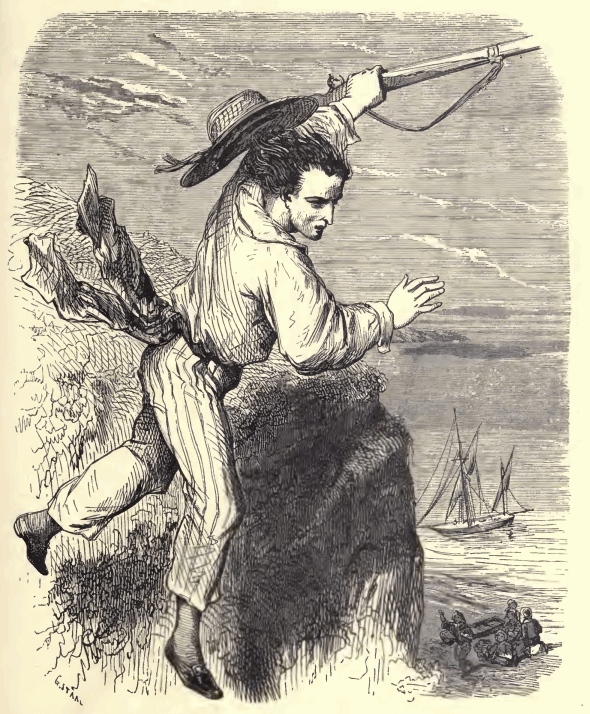
\includegraphics[width=\textwidth]{0295m.jpg}
\end{figure}

It seemed, however, to Edmond, who was hidden from his comrades by the
inequalities of the ground, that at sixty paces from the harbor the
marks ceased; nor did they terminate at any grotto. A large round rock,
placed solidly on its base, was the only spot to which they seemed to
lead. Edmond concluded that perhaps instead of having reached the end
of the route he had only explored its beginning, and he therefore
turned round and retraced his steps.

Meanwhile his comrades had prepared the repast, had got some water from
a spring, spread out the fruit and bread, and cooked the kid. Just at
the moment when they were taking the dainty animal from the spit, they
saw Edmond springing with the boldness of a chamois from rock to rock,
and they fired the signal agreed upon. The sportsman instantly changed
his direction, and ran quickly towards them. But even while they
watched his daring progress, Edmond’s foot slipped, and they saw him
stagger on the edge of a rock and disappear. They all rushed towards
him, for all loved Edmond in spite of his superiority; yet Jacopo
reached him first.

He found Edmond lying prone, bleeding, and almost senseless. He had
rolled down a declivity of twelve or fifteen feet. They poured a little
rum down his throat, and this remedy which had before been so
beneficial to him, produced the same effect as formerly. Edmond opened
his eyes, complained of great pain in his knee, a feeling of heaviness
in his head, and severe pains in his loins. They wished to carry him to
the shore; but when they touched him, although under Jacopo’s
directions, he declared, with heavy groans, that he could not bear to
be moved.

It may be supposed that Dantès did not now think of his dinner, but he
insisted that his comrades, who had not his reasons for fasting, should
have their meal. As for himself, he declared that he had only need of a
little rest, and that when they returned he should be easier. The
sailors did not require much urging. They were hungry, and the smell of
the roasted kid was very savory, and your tars are not very
ceremonious. An hour afterwards they returned. All that Edmond had been
able to do was to drag himself about a dozen paces forward to lean
against a moss-grown rock.

But, instead of growing easier, Dantès’ pains appeared to increase in
violence. The old patron, who was obliged to sail in the morning in
order to land his cargo on the frontiers of Piedmont and France,
between Nice and Fréjus, urged Dantès to try and rise. Edmond made
great exertions in order to comply; but at each effort he fell back,
moaning and turning pale.

“He has broken his ribs,” said the commander, in a low voice. “No
matter; he is an excellent fellow, and we must not leave him. We will
try and carry him on board the tartan.”

Dantès declared, however, that he would rather die where he was than
undergo the agony which the slightest movement cost him.

“Well,” said the patron, “let what may happen, it shall never be said
that we deserted a good comrade like you. We will not go till evening.”

This very much astonished the sailors, although, not one opposed it.
The patron was so strict that this was the first time they had ever
seen him give up an enterprise, or even delay in its execution. Dantès
would not allow that any such infraction of regular and proper rules
should be made in his favor.

“No, no,” he said to the patron, “I was awkward, and it is just that I
pay the penalty of my clumsiness. Leave me a small supply of biscuit, a
gun, powder, and balls, to kill the kids or defend myself at need, and
a pickaxe, that I may build a shelter if you delay in coming back for
me.”

“But you’ll die of hunger,” said the patron.

“I would rather do so,” was Edmond’s reply, “than suffer the
inexpressible agonies which the slightest movement causes me.”

The patron turned towards his vessel, which was rolling on the swell in
the little harbor, and, with sails partly set, would be ready for sea
when her toilet should be completed.

“What are we to do, Maltese?” asked the captain. “We cannot leave you
here so, and yet we cannot stay.”

“Go, go!” exclaimed Dantès.

“We shall be absent at least a week,” said the patron, “and then we
must run out of our course to come here and take you up again.”

“Why,” said Dantès, “if in two or three days you hail any fishing-boat,
desire them to come here to me. I will pay twenty-five piastres for my
passage back to Leghorn. If you do not come across one, return for me.”
The patron shook his head.

“Listen, Captain Baldi; there’s one way of settling this,” said Jacopo.
“Do you go, and I will stay and take care of the wounded man.”

“And give up your share of the venture,” said Edmond, “to remain with
me?”

“Yes,” said Jacopo, “and without any hesitation.”

“You are a good fellow and a kind-hearted messmate,” replied Edmond,
“and heaven will recompense you for your generous intentions; but I do
not wish anyone to stay with me. A day or two of rest will set me up,
and I hope I shall find among the rocks certain herbs most excellent
for bruises.”

A peculiar smile passed over Dantès’ lips; he squeezed Jacopo’s hand
warmly, but nothing could shake his determination to remain—and remain
alone.

The smugglers left with Edmond what he had requested and set sail, but
not without turning about several times, and each time making signs of
a cordial farewell, to which Edmond replied with his hand only, as if
he could not move the rest of his body.

Then, when they had disappeared, he said with a smile,—“’Tis strange
that it should be among such men that we find proofs of friendship and
devotion.” Then he dragged himself cautiously to the top of a rock,
from which he had a full view of the sea, and thence he saw the tartan
complete her preparations for sailing, weigh anchor, and, balancing
herself as gracefully as a water-fowl ere it takes to the wing, set
sail.

At the end of an hour she was completely out of sight; at least, it was
impossible for the wounded man to see her any longer from the spot
where he was. Then Dantès rose more agile and light than the kid among
the myrtles and shrubs of these wild rocks, took his gun in one hand,
his pickaxe in the other, and hastened towards the rock on which the
marks he had noted terminated.

“And now,” he exclaimed, remembering the tale of the Arabian fisherman,
which Faria had related to him, “now, Open Sesame!”
